\documentclass{standalone}
\usepackage{tikz}
\begin{document}
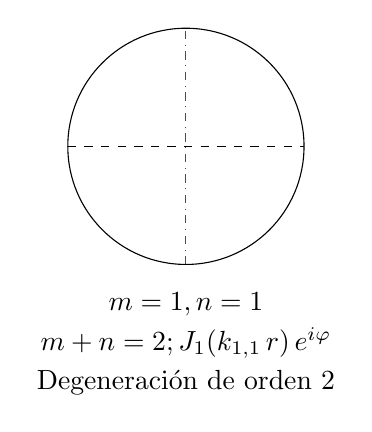
\begin{tikzpicture}
    \draw (0, 0) circle (1.5cm);
    \draw [dashed] (-1.5, 0) -- (1.5, 0);
    \draw [dash dot, color=red] (0, -1.5) -- (0, 1.5);
    \node at (0, -2) {$m = 1, n = 1$};
    \node at (0, -2.5) {$m + n = 2; J_{1}(k_{1,1} \, r) \, e^{i \varphi}$};
    \node at (0, -3) {Degeneración de orden 2};
\end{tikzpicture}
\end{document}